
\documentclass[12pt]{article}
\usepackage[spanish]{babel}
\usepackage{booktabs}
\usepackage{longtable}
\usepackage{latexsym}
\usepackage{lipsum}
\usepackage{graphicx}
\usepackage{setspace}
\usepackage{xcolor}

\textwidth     =  6.5in
\textheight    =  9.0in
\oddsidemargin =  0.2in
\topmargin     = -0.6in
\usepackage{amsmath, amssymb, latexsym}


%%%%%%%%%%%%%%%%%%%%%%%%%%%%%%%%%%%%%%%%%%%%%%%%%%%%%%%%%%%%%%%%%%%%%%%%
\newcommand{\be}{\begin{equation}}
\newcommand{\ee}{\end{equation}}
\newcommand{\bes}{\begin{equation*}}
\newcommand{\ees}{\end{equation*}}

\newcommand{\bea}{\begin{eqnarray}}
\newcommand{\eea}{\end{eqnarray}}

\newcommand{\beas}{\begin{eqnarray*}}
\newcommand{\eeas}{\end{eqnarray*}}

\newcommand{\bet}{\begin{tabular}}
\newcommand{\ent}{\end{tabular}}
\newcommand{\mul}{\multicolumn}
\newcommand{\bec}{\begin{center}}
\newcommand{\enc}{\end{center}}
\newcommand{\bei}{\begin{itemize}}
\newcommand{\eni}{\end{itemize}}
\newcommand{\bee}{\begin{enumerate}}
\newcommand{\ene}{\end{enumerate}}
\newcommand{\noi}{\noindent}
\newcommand{\unl}{\underline}
\newcommand{\ul}{\underline}
\newcommand{\real}{\mathbb{R}}
\newcommand{\feal}{\mathbb{F}}
\newcommand{\natu}{\mathbb{N}}
\newcommand{\fact}{\mathbb{X}}

\begin{document}

\title{Optimizaci\'on num\'erica}
\author{Proyecto final 1. PCS (GCP+RC)}
\date{ Santiago Novoa P\'erez. 8 de diciembre del 2015.}
\maketitle


\subsubsection*{Introducci\'on}
\noi El m\'etodo de programaci\'on cuadr\'atica sucesiva (PCS) es uno de los m\'etodos m\'as efectivos para resolver problemas de optimizaci\'on no lineales. Para que el m\'etodo funcione se necesita que tanto la funci\'on objetivo como las restricciones sean dos veces continuamente diferenciables.\\
 
  Los m\'etodos PCS resuelven una secuencia de subproblemas de optimizaci\'on en la que, en cada subproblema, se intenta resolver un modelo cuadr\'atico de la funci\'on objetivo sujeta a una linealizaci\'on de las restricciones; puede ser utilizado tanto con un marco de regiones de confianza como uno de b\'usqueda lineal.\\
 
  En general los m\'etodos PCS se pueden ver como una generalizaci\'on del m\'etodo de Newton para optimizaci\'on sin restricciones dado a la manera en que encuentran una direcci\'on de descenso.\\
 
  PCS es apropiado para problemas grandes y peque\~nos con funciones no lineales; en estos casos la soluci\'on se alcanza en un n\'umero de iteraciones sustancialmente menor que $n$.\\
  
  Uno de los problemas que encuentra el m\'etodo de PCS es que al enfrentarse a regiones donde las matrices no tienen la curvatura deseada (tienen curvatura negativa o cero) el algoritmo se sale de lugar y no puede converger. Existen muchas formas de tratar estos problemas, ya sea con regularizaci\'on o incorpor\'andole GC al m\'etodo para siempre tener direcciones de descenso. \\
  
  Para este proyecto en particular, nos interesar\'a volver el m\'etodo local de PCS (por problemas de inercia) en un m\'etodo global incorporando regiones de confianza. Para entender mejor c\'omo funcionan las regiones de confianza en problemas con restricciones, incorporaremos el algoritmo dogleg a un m\'etodo de gradiente conjugado proyectado con regi\'on de confianza, intentando, as\'i, resolver el problema de la inercia en muchos de los problemas de PCS de una vez por todas. \\
  
  El problema que buscamos resolver es:
  \beas
  {\text {minimizar}}\ &\ f(x)\\
  {\text {s.a.}}\ \ &\  c(x) = 0 \\ \\
  f: \real^n &\longrightarrow \real \\
  c: \real^n &\longrightarrow \real^m \ \ \  \\
  \Omega = \{x \in \real^n\ |&c(x) = 0\}\\
  \eeas
  Sin embargo, aplicando regiones de confianza, el problema que trataremos ser\'a:
  \beas
  {\text {minimizar}}\ &\ f(x)+\nabla f(x)^Tp + \frac{1}{2}p^T\nabla_{xx}^2\mathcal{L}p\\
  {\text {s.a.}}\ \ &\  A(x)p+c(x) = 0 \\
  &\|p\|\leq \Delta
  \eeas
\noi El problema anterior es un problema cuadr\'atico que se puede resolver usando Gradiente Conjugado Proyectado. Lo que hace GCP es resolver el problema de minimizar 
$$$$

 \subsubsection*{Construcci\'on del m\'etodo}
 \bei
 \item Condiciones de Optimalidad
 \eni
 Sean
 \beas
 \L(x,\lambda) = f(x) - \lambda^Tc(x)\\
 A(x) = \left[\nabla c_i^T(x)\right]_{i=1...m}
 \eeas
$$$$

Si $x^*$ es minimizador local de $f$, entonces $\exists$ $\lambda^*$ tal que:\\
\beas
\nabla_x\L(x^*,\lambda^*) = \nabla f(x^*) - &\sum_{i=1}^m {\lambda_i}^*\nabla c_i(x^*)\\=& 0;\\ 
\nabla_\lambda\L(x^*,\lambda^*) =& c(x^*)\\
=&0;
\eeas
Estas ecuaciones resultan de intentar ver en d\'onde el gradiente de la funci\'on lagrangiana se anula para poder encontrar el m\'inimo de esa funci\'on (condiciones necesarias de primer orden).\\

Si adem\'as los gradientes de las restricciones son L.I. (complementariedad estricta), entonces el cono cr\'itico y el espacio nulo de A son el mismo y podemos ver la convexidad de $\L$ en: 
\beas
w^T\nabla_{xx} \L(x^*,\lambda^*)w\  \geq\  0\ \ \ \  \forall w \in C(x^*,\lambda^*) 
\eeas
\noi con $C(x^*,\lambda^*)$ el cono cr\'itico en $x^*$ , $\lambda^*$, que son todas las direcciones que cumplen con que mantienen las restricciones (en una aproximaci\'on lineal) cercanas a factibilidad, es decir:
\beas
C(x^*,\lambda^*)= \{w \in \real^n\ |\ \nabla c_i(x^*)^Tw = 0\ \ \forall i \in \{1,...,m\}\}
\eeas
Lo que esto asegura es que cuando el gradiente s\'i se anule,o la direcci\'on que se tome sea de descenso o todas las direcciones sean de ascenso ( usando la expansi\'on de Taylor y el Lema de Farkas: estar en el cono ( con su respectivo $\lambda$ ) o que exista descenso). Tambi\'en se les conoce como condiciones necesarias de segundo orden.\\
Si queremos asegurar que el problema (convexo) va a encontrar su m\'inimo en $x^*$ (condiciones suficientes de segundo orden), tenemos que ver que la Hessiana de la matriz Lagrangiana sea positiva definida en la proyecci\'on de las direcciones del cono cr\'itico:
\beas
0\ \textless\ w^T\nabla_{xx}\L(x^*,\lambda^*)w \ \ \ \ \forall\ w \in\  \{C(x^*,\lambda^*)\ \diagdown\ w=0\}
\eeas
\bei
\item M\'etodo cuadr\'atico
\eni
La matriz de KKT del problema anterior queda expresada como sigue: 
 \[
   K=
  \left[ {\begin{array}{cc}
   W_k\  &\  A^T(x_k) \\       A(x_k)\ &\ 0       \end{array} } \right]
\]
\noi donde $W_k$ es la matriz Hessiana de la funci\'on Lagrangiana del problema de optimizaci\'on.

La K es un resultado de escribir las condiciones de optimalidad descritas anteriormente en un sistema de ecuaciones:
 \[
  \left[ {\begin{array}{cc}
   W_k\  &\  A^T(x_k) \\       A(x_k)\ &\ 0       \end{array} } \right] * \left[{\begin{array}{c} h_x \\ -\lambda_{k+1}\end{array}}\right] = - \left[{\begin{array}{c}\nabla f(x_k) \\ c(x_k) \end{array}}\right]
\] \\
Es f\'acil verificar que resolver el sistema anterior es equivalente a resolver otro subproblema cuadr\'atico:
\beas
min\ \  \frac{1}{2}p^TQ_kp + g_k^Tp\\
s.a.\ \ \ A_k^Tp + c_k = 0
\eeas

Aqu\'i parece que se ha perdido el significado inicial del problema dado que se empez\'o hablando de $\nabla_{xx}\L(x_k)$ y de si su proyecci\'on en el espacio nulo de $A(x_k)$ (todas las direcciones en $C(x_k,\lambda_k)$ con k lo suficientemente grande para que $x_k$ y $\lambda_k$ se encuentren en el cono factible (una vecindad factible de la soluci\'on)) era positiva definida, sin embargo, gracias al resultado de un art\'iculo de Nicolas I.M. Gould \footnote{{\bf{Nicolas I.M. Gould}}; {\it{On practical conditions for the existence and uniqueness of solutions to the general equality quadratic programming problem}}}, este nuevo problema de optimizaci\'on tiene propiedades deseables. 
En primer lugar, si la proyecci\'on de la Hessiana de la Lagrangiana sobre el espacio nulo de los gradientes de las restricciones es SPD, la soluci\'on de los dos modelos existe y es \'unica.
Tambi\'en se prueba que el m\'inimo del problema de optimizaci\'on se puede calcular usando una base del espacio nulo.
Sin embargo, el resultado m\'as importante (por su practicidad) de la lectura vincula a la inercia de la Hessiana proyectada sobre el nulo con la inercia de K. 
\[
Z_k^T\nabla \L(x_k,\lambda_k)Z_k = Z_k^TW_kZ_k > 0\\ 
\]
\[
\implies\  \exists!\ p\ \  t.q.\ \  \\ 
{\text{p minimiza el problema cuadr\'atico}} \\ \]
\[
\therefore p {\text{\ minimiza al problema original}}\\
\]
\[
inercia(K)  = inercia(Z^TW_kZ^T) + (m,0,m)
\]
\[
\therefore inercia(K) = (m,0,n) \iff Z^TW_kZ^T {\text{\ es SPD}}
\]
\\
\noi La inercia de una matriz es una ternia que dice el n\'umero de valores propios menores a cero, cero y mayores a cero respectivamente : $$inercia (A) = (\lambda_{-}, \lambda_0, \lambda_{+})$$

Todos estos resultados nos aseguran que, si la inercia de la matriz K es la correcta $(m,0,n)$, resolver el problema de minimizaci\'on con restricciones de igualdad formulado al principio de este trabajo es equivalente a ir resolviendo una serie de subproblemas cuadr\'aticos convexos representados por las ecuaciones de KKT. Paso a paso ser\'a necesario resolver, para cada matriz K, el correspondiente vector h que resulte en el lado derecho de la ecuaci\'on. La soluci\'on (por ser un problema convexo), si las condiciones anteriores se cumplen, existir\'a paso a paso y ser\'a \'unica.
\[
K*h_k = LD = -\left[\begin{array}{c}\nabla f(x_k)\\ c(x_k)\end{array}\right]
\]

Este proceso parece ser igual de complicado que resolver el problema de minimizaci\'on del inicio, sin embargo, gracias a m\'etodos, como el programado en matlab llamado ldl, que factorizan matrices en matrices de bloques diagonales, es posible encontrar la inercia de una matriz y resolver sistemas de ecuaciones lineales sin que el costo computacional sea tan alto.  $$$$

 \subsubsection*{Convergencia global}
\noi Como dijimos anteriormente, regiones de confianza es una manera muy sencilla de asegurar que haya convergencia global, sin embargo, como estamos tratando con problemas con restricciones, las cosas se pueden complicar un poco. \\

El enfoque de regiones de confianza hace que al calcular la nueva direcci\'on se haga un acuerdo entre el paso a dar y la regi\'on dentro donde se da, si el acuerdo es malo la regi\'on se encoge, si el acuerdo es bueno (el paso es de descenso y no sales de factibilidad), la regi\'on se agranda. Para mantener a las restricciones en este acuerdo se usa a la funci\'on de m\'erito para hacer el modelo, sin embargo, para nuestra prueba s\'olo querremos ver qu\'e pasa con dogleg y GCP.\\

Otra dificultad que tienen regiones de confianza cuando tratan problemas con restricciones es que muchas veces no son compatibles las regiones con las restricciones. El primer pensamiento que usualmente surge con esto es agrandar la regi\'on para que incluya a las restricciones, pero eso ser\'ia una contradicci\'on al acuerdo y a c\'omo trabajan regiones de confianza. Una manera correcta de tratar con este problema es dividir al problema de minimizaci\'on en 2 subproblemas, uno inicial que nos otorge una r con la cu\'al vamos a relajar nuestras restricciones (dogleg hace esto) y otro que resuleva GCP ya con las nuevas condiciones.\\
  \beas
  {\text {minimizar}}\ &\ f(x)+\nabla f(x)^Tp + \frac{1}{2}p^T\nabla_{xx}^2\mathcal{L}p\\
  {\text {s.a.}}\ \ &\  A(x)p+c(x) = r_k \\
 & r_k = A_kv^{*} + c_k\\
  &\|p\|\leq \Delta
  \eeas
\noi Este sistema relajado tiene que resolver primero el para el valor de $v^*:$
  \beas
  {\text {minimizar}}\ &\ \|A_kv + c_k\|\\
  &\|v\|\leq 0.8\Delta_k
  \eeas
  \begin{center}
\begin{figure}[!htb]
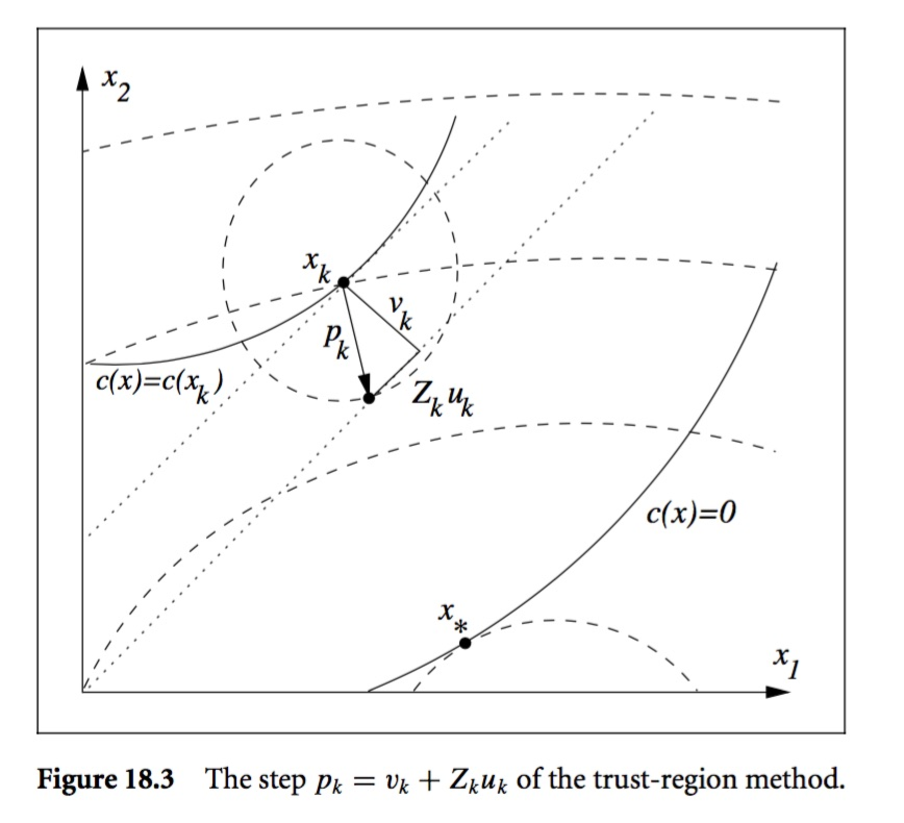
\includegraphics[scale = 0.75]{dogleg_trust_region}
\end{figure}
\end{center}
  Para calcular cu\'anto va a relajar las restricciones, dogleg usa dos direcciones, la direcci\'on de Cauchy ($p^U$) y la direcci\'on de Newton o el paso completo ($p^N$). Despu\'es de calcular las dos direcciones avanza completamente en la direcci\'on de Cauchy y al final de ella le pega la direcci\'on de Newton formando as\'i una curva parametrizada de $x_0$ hasta el final de la direcci\'on de Newton. Lo que hace despu\'es es cortar ese segmento creado en donde \'este corte con la regi\'on de confianza:
\begin{center}
\begin{figure}[!htb]
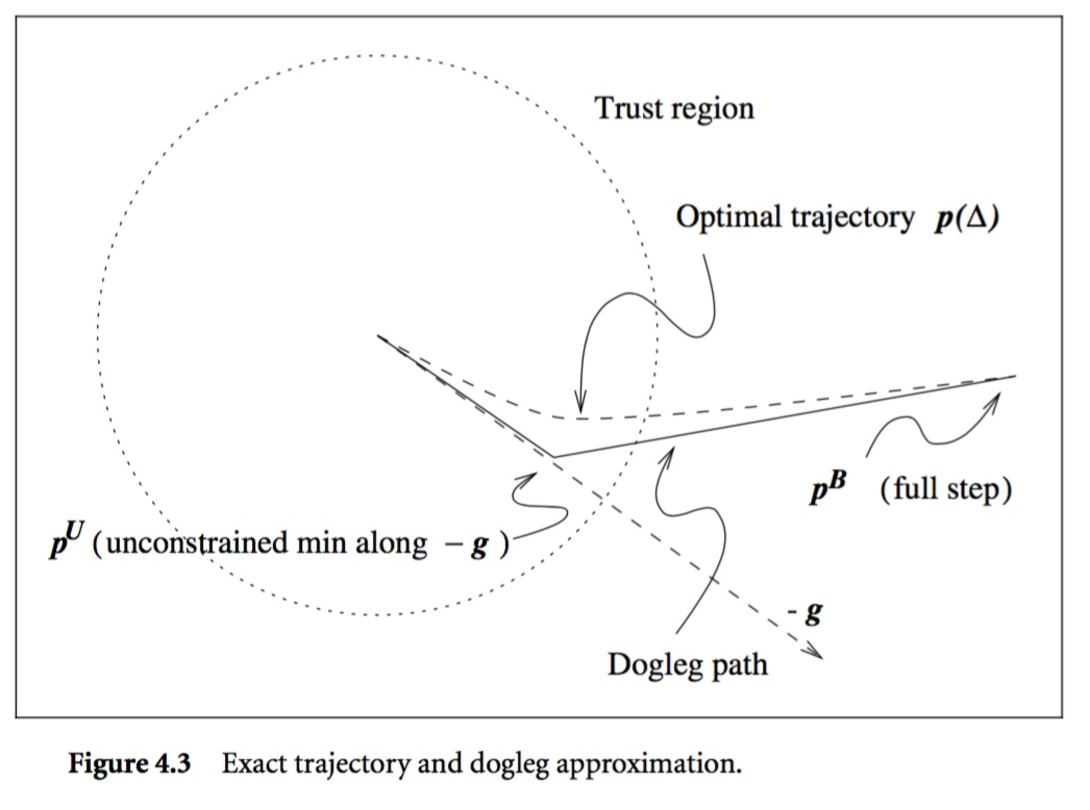
\includegraphics[scale = 0.75]{dogleg}
\end{figure}
\end{center}
\noi Este proceso nos deja con 2 posibles resultados:
\bei
\item La regi\'on de confianza corta antes de que empiece el paso de Newton, lo cual quiere decir que el paso de Newton solito est\'a dando un avance mayor a lo que la regi\'on de confianza acepta por lo que ser\'ia conveniente ver si el acuerdo es bueno y tal vez agrandar la regi\'on.
\item La regi\'on de confianza corta a la direcci\'on despu\'es de que el segmento de recta di\'o vuelta y tal vez las direcciones obtenidas en esta regi\'on no son las mejores por lo que podr\'ia convenir recortar la regi\'on.
\eni
 \pagebreak
\subsubsection*{Experimento} 
\bee
\item Constantes $c_1 = 10^{-4}$ ,   $maxiter = 1000$ ,  $TOL = 10^{-7}$
\item Condiciones de paro
\beas
k \geq& maxiter\\
\sqrt{|{r_k}^T*y_k|}\leq& TOL(r_0^T*y_0))
\eeas
\item Reporte del experimento
\ene
{\tiny{\setstretch{0.8}\color{gray}
\begin{table}[htbp]
  \centering
  \caption{Matrices Poisson con GCP+RC}
    \begin{tabular}{rrrrrrrrrr}
    \toprule
    n     & m     & $\|\Delta\|$ & $\|res\|$ & $\|p\|\geq\|\Delta\|$ & $\|p\|$ & iter  & CPU(s) & err rel & fact pr \\
    \midrule
    10000 & 100   & 1     & 3.40E+00 & TRUE  & 1     & 0     & 9.65E-03 & 1.00E+00 & 1.59E-17 \\
    10000 & 200   & 1     & 3.68E+00 & TRUE  & 1     & 0     & 1.40E-02 & 1.00E+00 & 2.78E-17 \\
    10000 & 9900  & 1     & 7.05E+00 & TRUE  & 1     & 0     & 6.02E-01 & 1.00E+00 & 2.90E-15 \\\hline
    10000 & 100   & 25    & 1.03E+01 & TRUE  & 25    & 26    & 2.85E-02 & 6.72E-02 & 7.23E-15 \\
    10000 & 200   & 25    & 1.04E+01 & TRUE  & 25    & 27    & 2.40E-01 & 6.39E-02 & 2.45E-14 \\
    10000 & 9900  & 25    & 1.14E+01 & FALSE & 22.3508 & 33    & 1.88E+00 & 1.97E-06 & 5.90E-14 \\\hline
    10000 & 100   & 125   & 1.03E+01 & FALSE & 49.7498 & 193   & 1.91E-01 & 1.08E-06 & 8.74E-14 \\
    10000 & 200   & 125   & 1.04E+01 & FALSE & 49.5547 & 205   & 1.88E+00 & 1.00E-06 & 3.58E-13 \\
    10000 & 9900  & 125   & 1.74E+01 & FALSE & 36.2494 & 33    & 1.68E+00 & 2.00E-06 & 9.81E-14 \\\hline
    10000 & 100   & 10000 & 10.29563 & FALSE & 49.7498 & 193   & 0.1901534 & 1.0789E-06 & 8.7359E-14 \\
    10000 & 200   & 10000 & 10.3923 & FALSE & 49.5547 & 205   & 1.737791 & 1.0013E-06 & 3.576E-13 \\
    10000 & 9900  & 10000 & 17.37815 & FALSE & 36.2494 & 33    & 1.75811 & 1.9995E-06 & 9.8137E-14 \\
    \bottomrule
    \end{tabular}%
  \label{tab:addlabel}%
\end{table}%
}}
\subsubsection*{Observaciones}
\bee
\item Para probar el algoritmo lo \'unico que se hizo fue agarrar diferentes tama�os para la regi\'on inicial y ver si alguna de las direcciones chocaba con la regi\'on antes de otorgar una respuesta por GCP.
\item Todas las iteraciones tienen curvatura positiva ya que elegimos probar el algoritmo con matrices Poisson.
\item Como todas las iteraciones est\'an en regiones de curvatura positiva, los pasos tomados son grandes en general, es decir, se agrandar\'ia la $\Delta$ en el siguiente paso para la mayor\'ia de condiciones iniciales que se consideran en problemas de este tipo ($\Delta=1$ es una regi\'on usual para empezar).
\item Como cortamos el algoritmo una vez que la direcci\'on chocara con la regi\'on (para no tener que calcular el acuerdo), podemos ver como baja el error una vez que el algoritmo corre y termina (s\'olo hay que fijarse en la diferencia entre las primeras 3 iteraciones y las \'ultimas 6 donde el resultado s\'i es un minimizador local).
\item Las direcciones que dogleg arroja (res) tambi\'en van creciendo conforme la regi\'on crece, sin embargo parece que depende tambi\'en del precondicionador que se est\'e usando, es decir, d\'onde se est\'a proyectando el problema.
\ene

\end{document}  